\chapter{Progettazione e codifica}

\label{cap:progettazione}

\intro{Durante la fase di progettazione viene definita l'architettura del software, questa operazione consiste nella suddivisione del sistema in componenti distinti, ognuno con compiti differenti.
L'obiettivo è pianificare in maniera chiara tutte le azioni che l'applicativo dovrà svolgere prima di passare effettivamente alla codifica.}

\section{Architettura}
L'architettura (Fig.~\ref{fig:schema-architettura})pensata prevede l'utilizzo di 4 componenti principali che si occupano di:
\begin{enumerate}
    \item Acquisire gli screenshot.
    \item Effettuare il clustering degli screenshot acquisiti.
    \item Valutare i siti web.
    \item Inviare e-mail promozionali.
\end{enumerate}

\begin{figure}[!h] 
    \centering 
    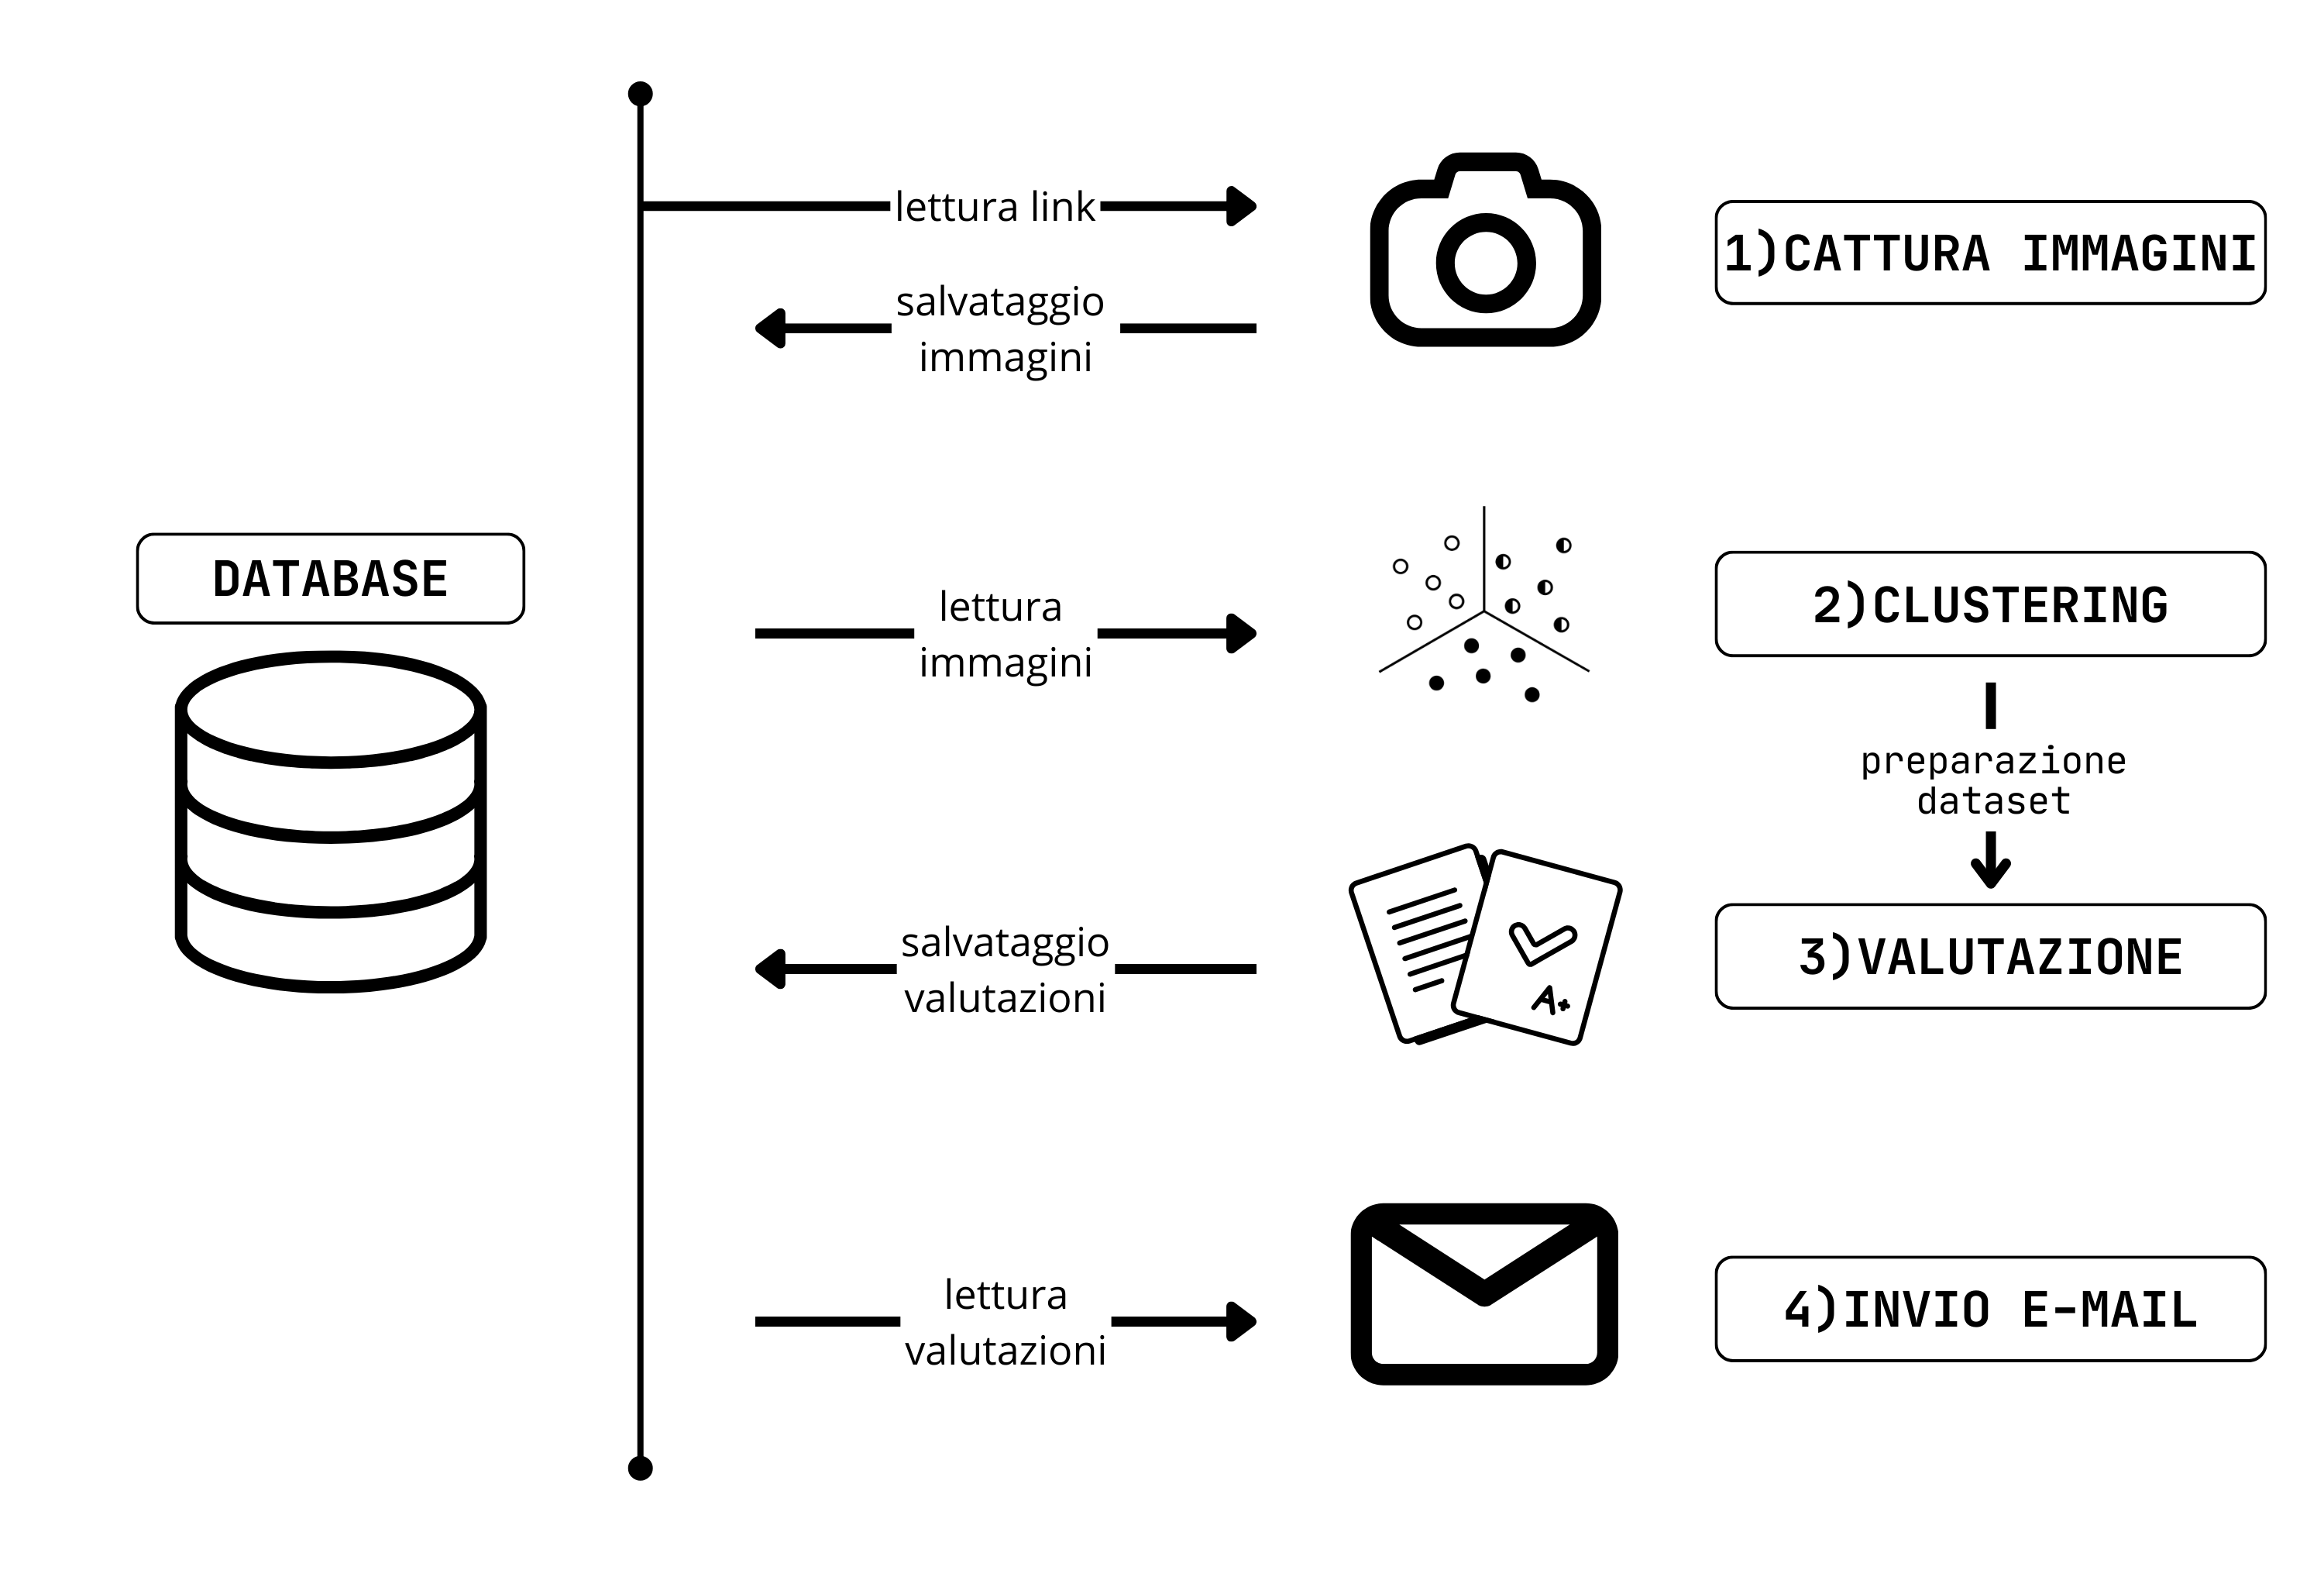
\includegraphics[width=0.9\columnwidth]{progettazione/schema-architettura.png} 
    \caption{Schema architetturale del progetto}
    \label{fig:schema-architettura}
  \end{figure}


\newpage

\section{Cattura immagini}

\section{Clustering}

\section{Valutazione}

\section{Invio e-mail}

\section{Database}